\documentclass{exam}
\usepackage{mainExam}

\title{Interrogation : nombre dérivé}
\date{16 Mai 2024}
\author{Maths Spécifiques}

\begin{document}
\maketitle
\thispagestyle{head}
\begin{questions}
\titledquestion{Tangentes}[4]
Soit $f$ une fonction définie sur $\R$ dont la courbe représentative $\mathcal{C}_f$ est donnée ci-après.
\begin{center}
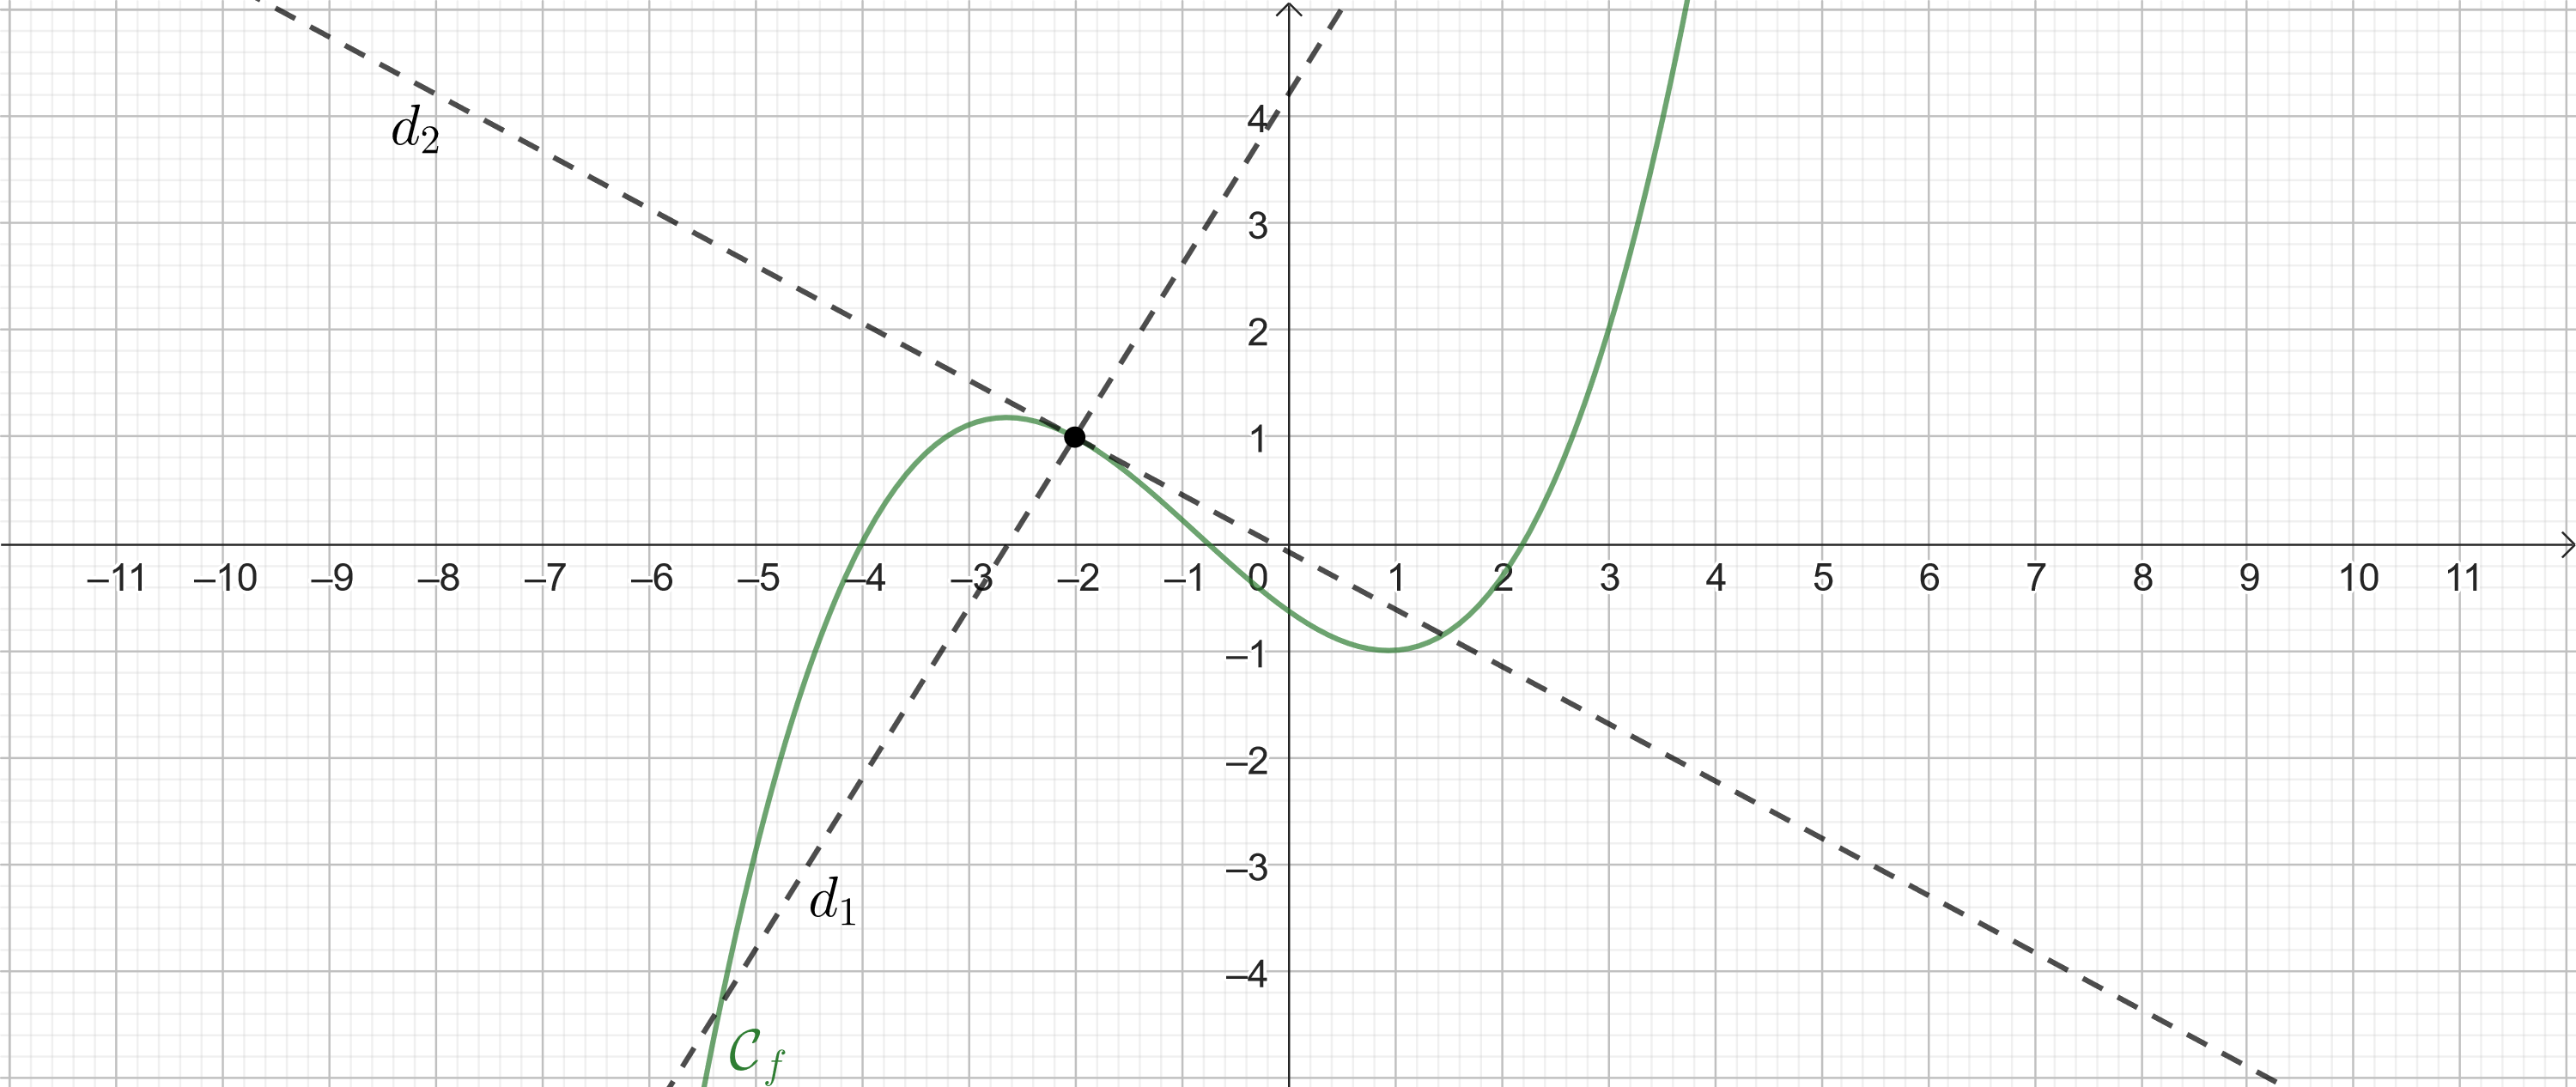
\includegraphics[width=0.9\textwidth]{Exo1.png}
\end{center}
\begin{parts}
\part Deux droites $d_1$ et $d_2$ ont été représentées en pointillés. Laquelle est une tangente à la courbe $\mathcal{C}_f$ ?
\part Tracer une tangente à $\mathcal{C}_f$ en $A(0;f(0))$.
\end{parts}
\makeemptybox{2cm}
\titledquestion{Nombre dérivé}[4]
Soit $f$ une fonction définie sur $\R$. Sa courbe représentative $\mathcal{C}_f$ ainsi qu'une de ses tangentes $t$ sont données par la figure ci-contre.
\begin{center}
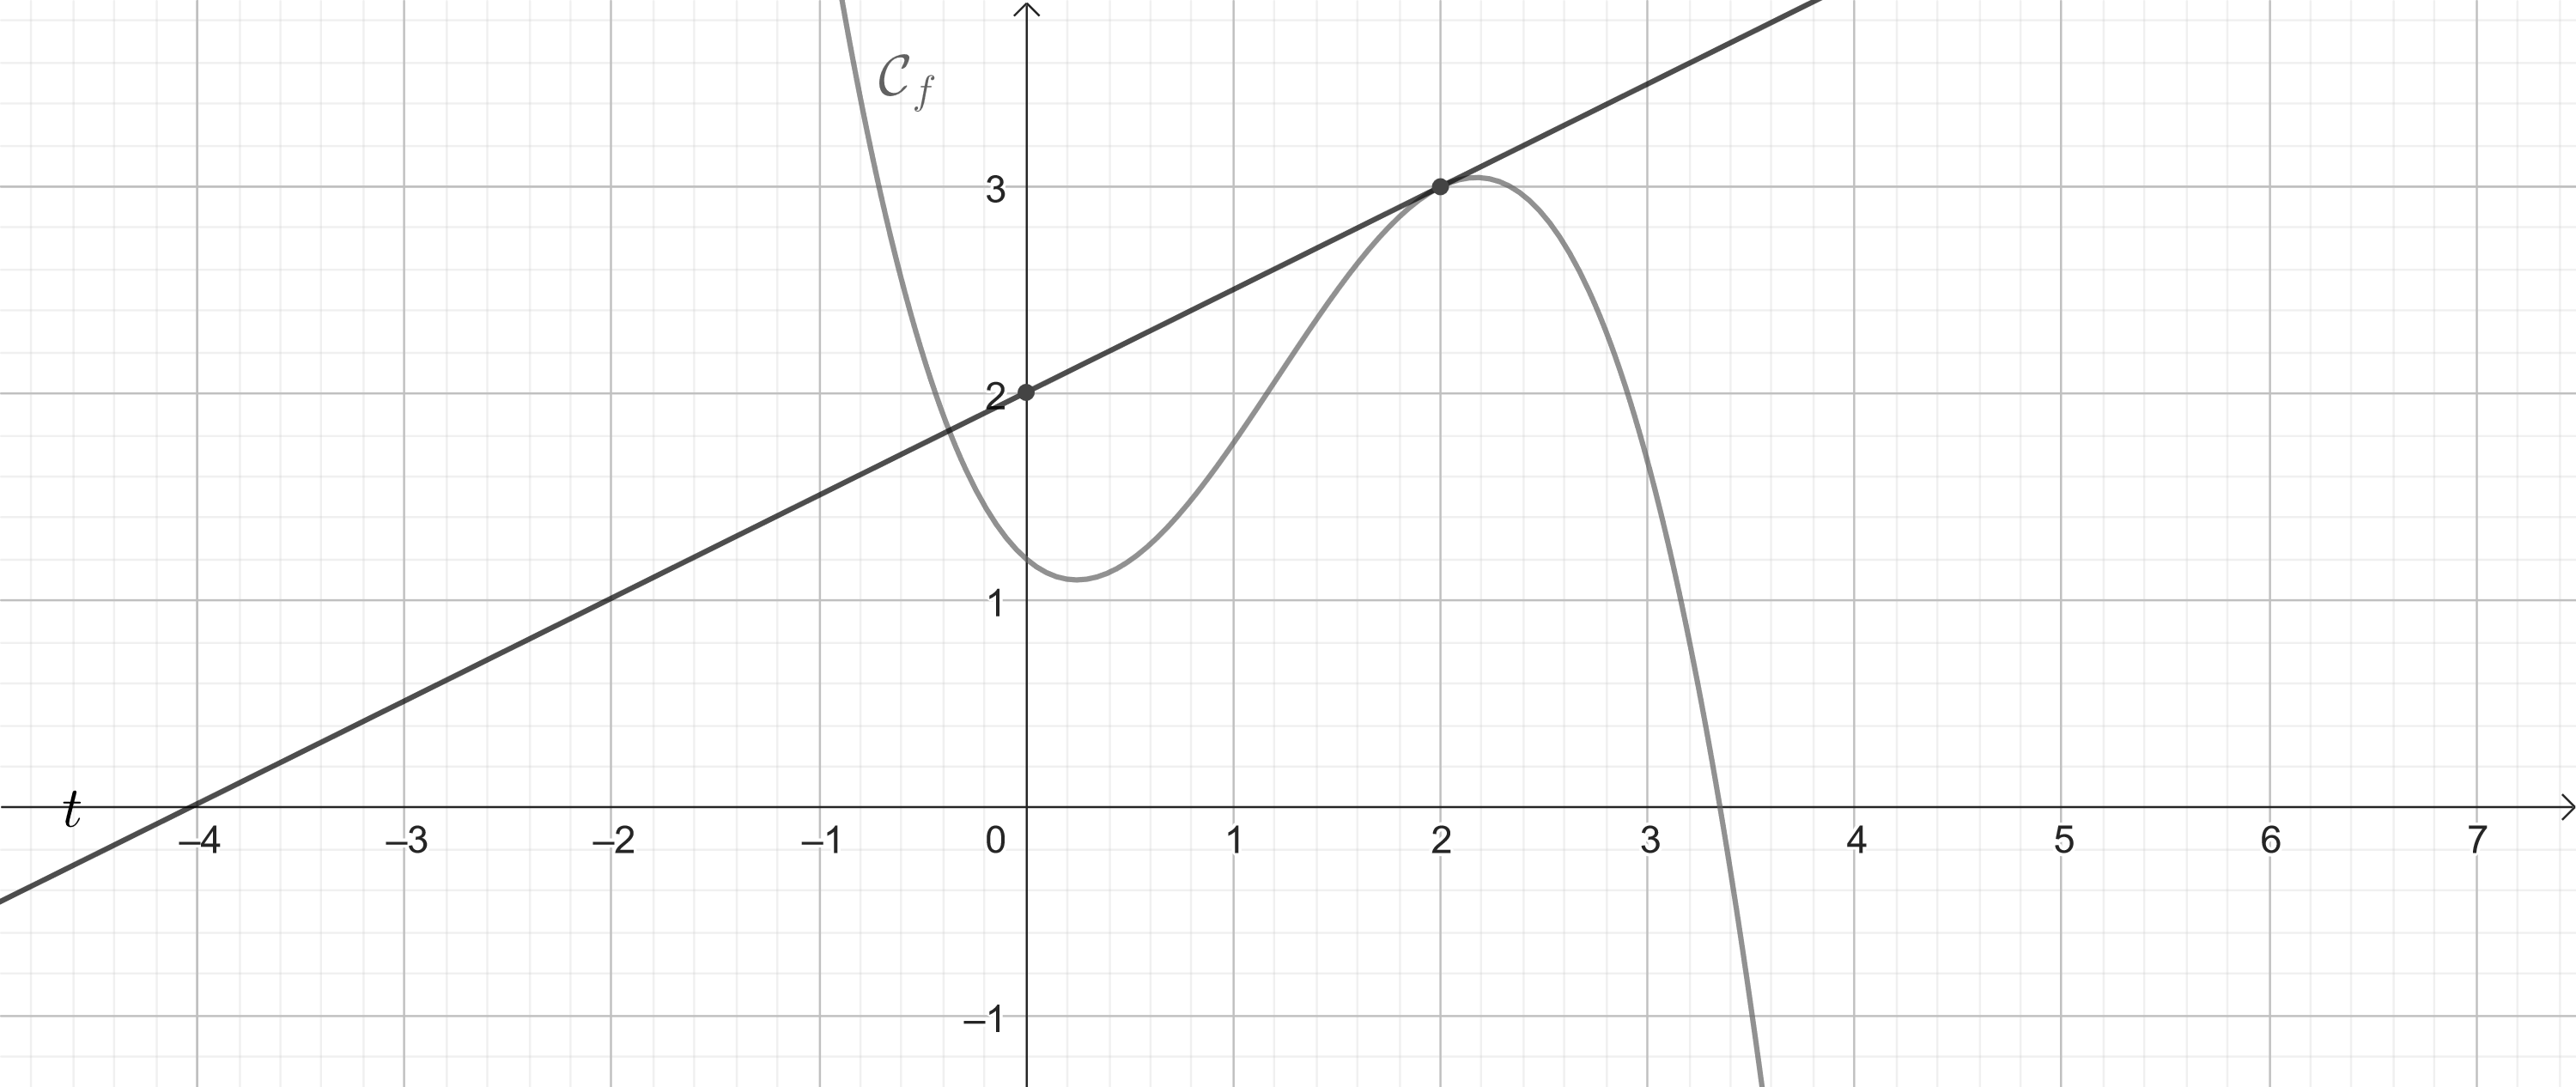
\includegraphics[width=0.9\textwidth]{Exo2.png}
\end{center}
\begin{parts}
\part En quel point de la courbe la droite $t$ est-elle une tangente à $\mathcal{C}_f$ ?
\part En déduire le nombre dérivé de $f$ en $2$. 
\end{parts}
\makeemptybox{4cm}
\question[2]
L'allure de la rampe d'un skatepark est modélisée par une fonction $f$ dont la courbe représentative est donnée ci-contre.
\begin{center}
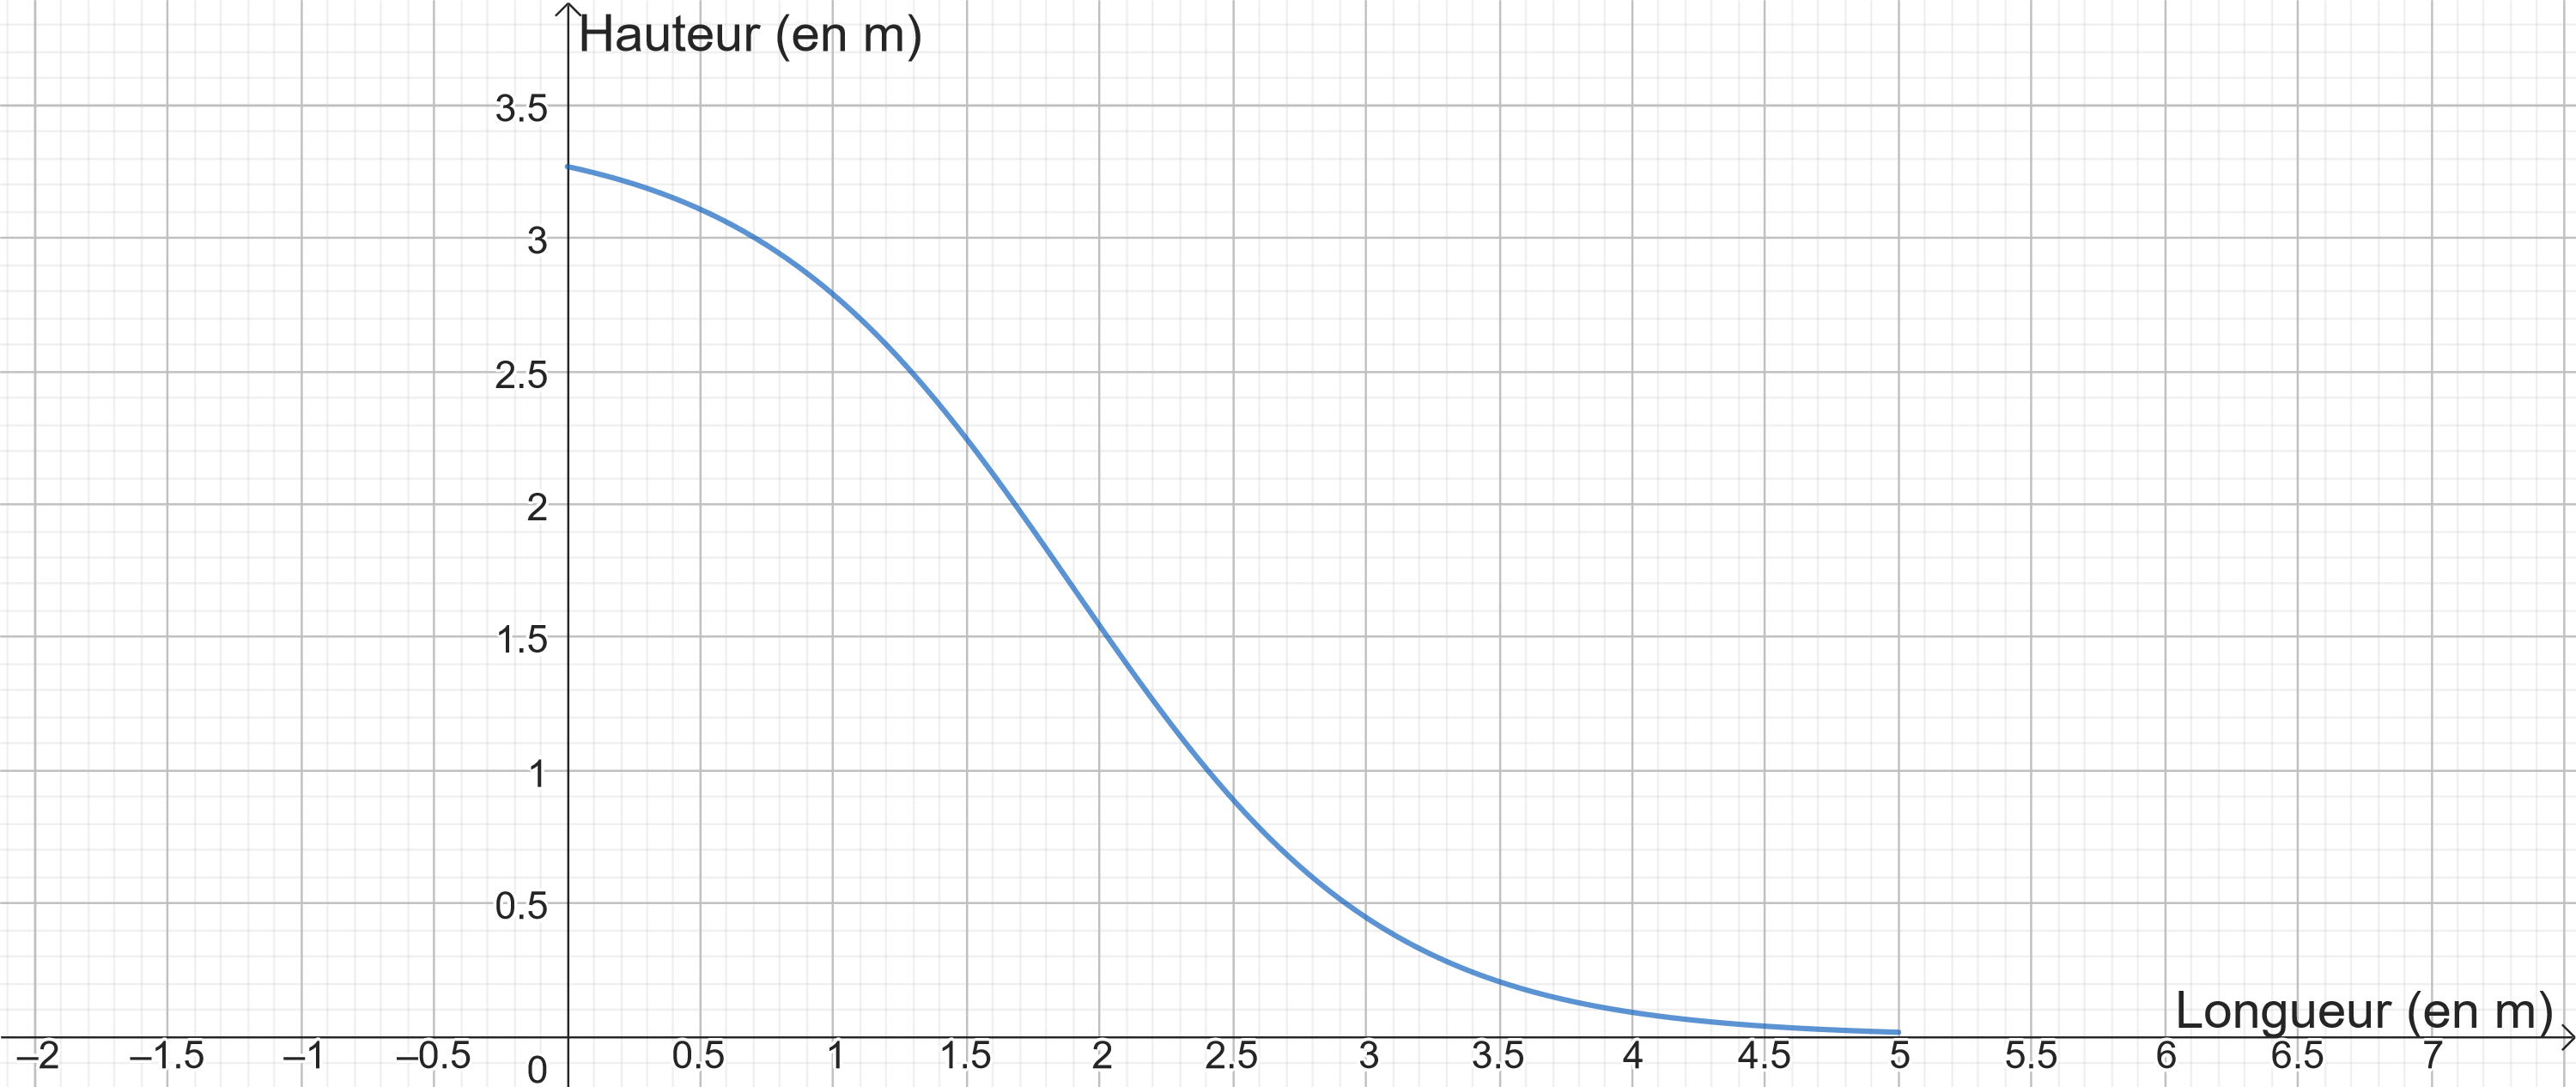
\includegraphics[width=0.9\textwidth]{Exo3.png}
\end{center}
\begin{parts}
\part À quelle longueur et à quelle hauteur la pente est-elle la plus raide ?
\part Quelle interprétation avoir sur le nombre dérivé de $f$ en cette longueur ?
\end{parts}
\makeemptybox{4cm}
\end{questions}
\end{document}